\begin{frame}\frametitle{ \vspace*{0.5cm} Results: Dependence of interface dynamics on wave duration}
  \begin{figure}
    \centering
    \hfill%
    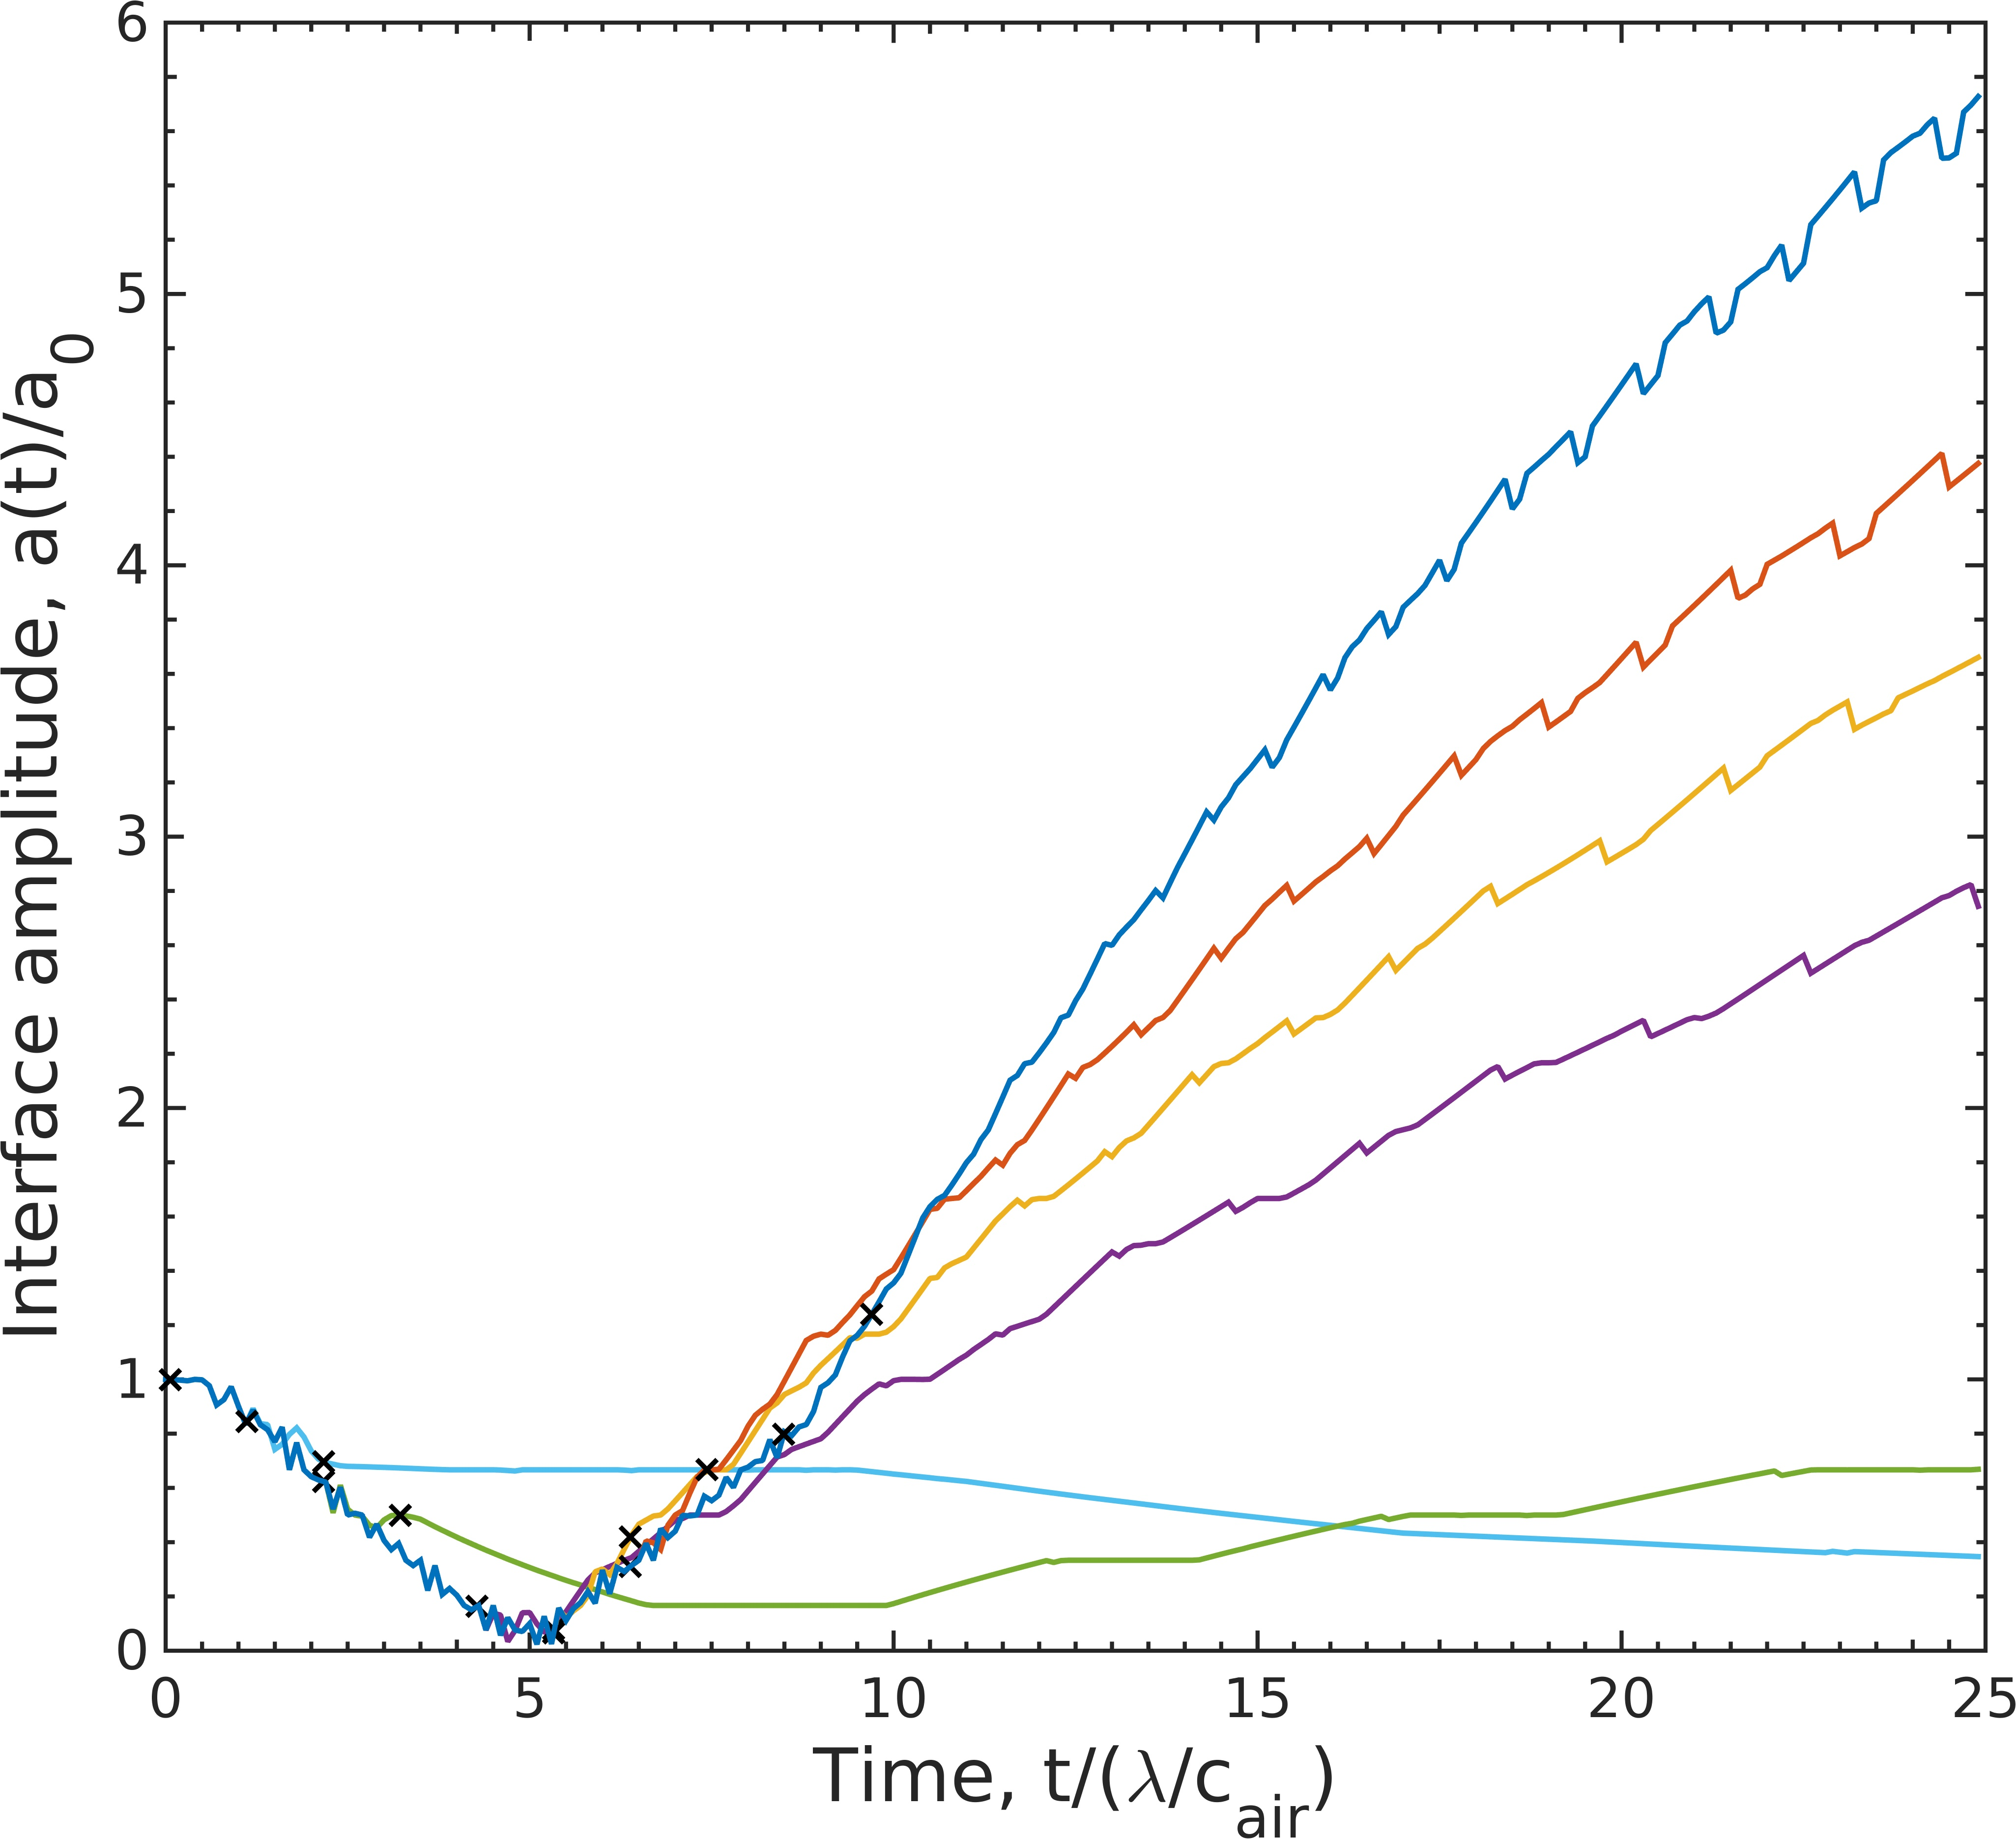
\includegraphics[height=0.52\textheight]{../figs/lung_figs/interface_multi-lag}\hfill%
    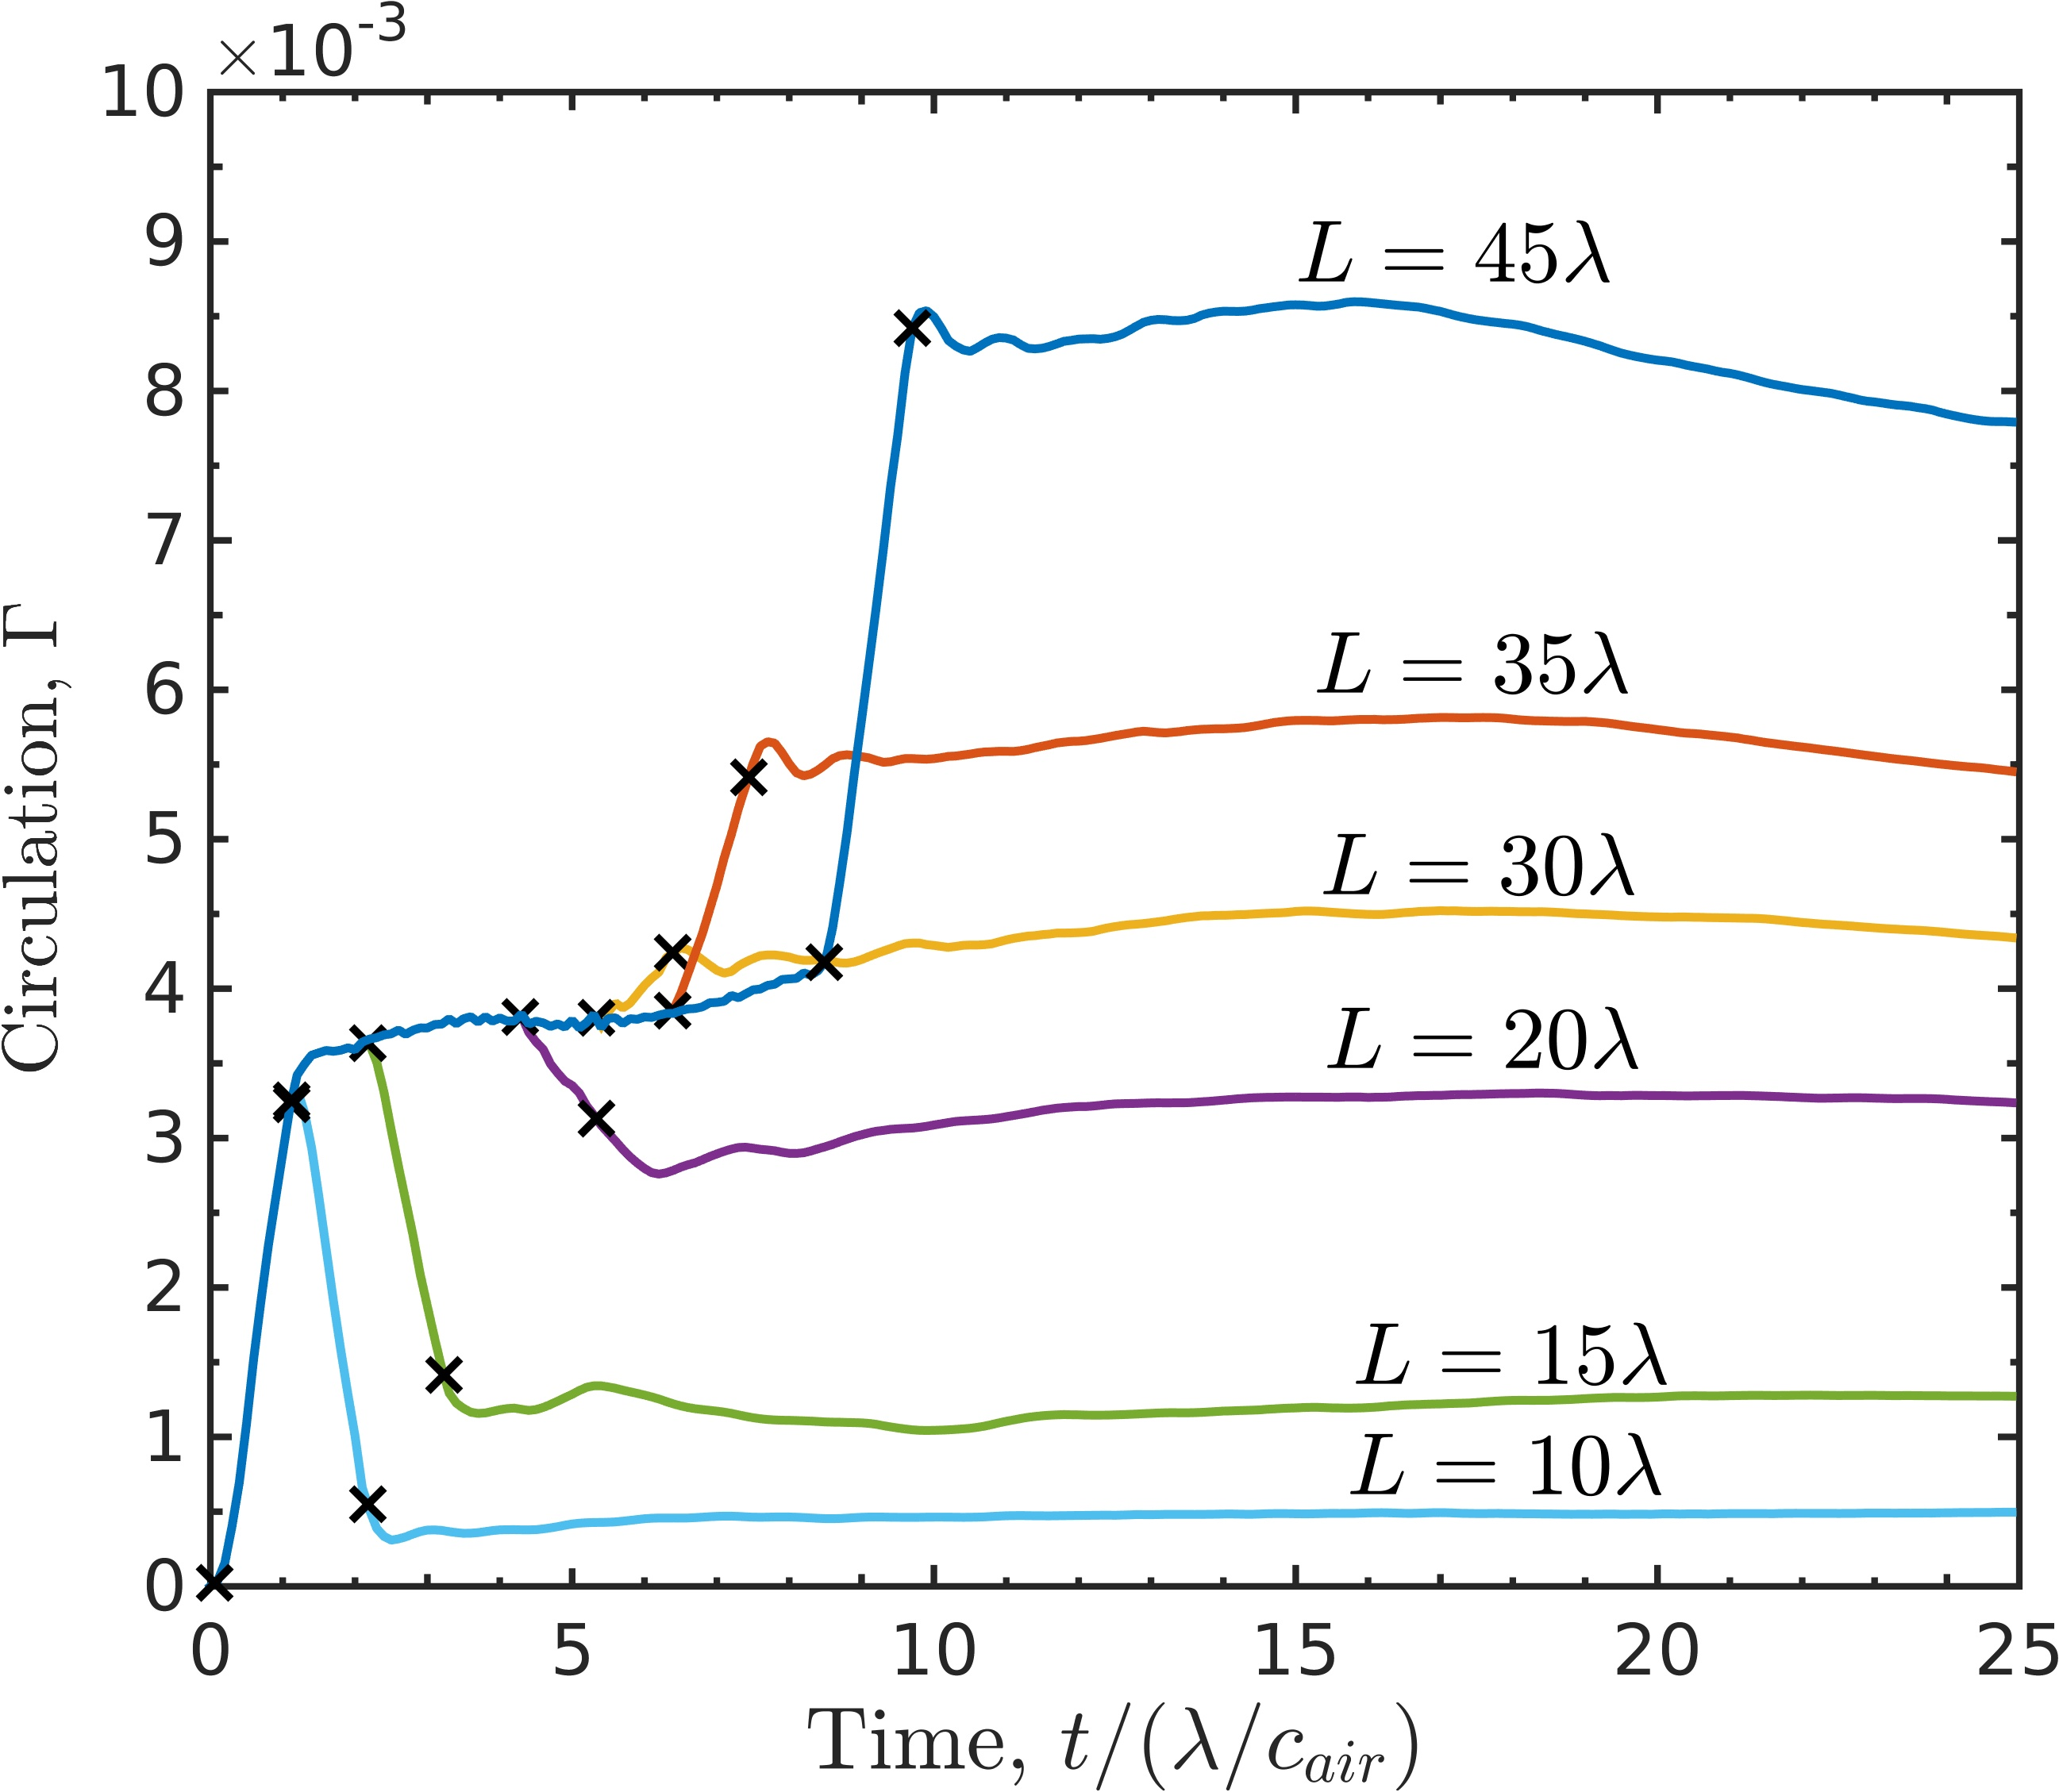
\includegraphics[height=0.53\textheight]{../figs/lung_figs/circulation_multi-lag_fixed}%
    \hfill%
  \end{figure}
  \begin{itemize}
  \item Changing wave width changes time when expansion hits interface.
  \item Time-dependent interface deformation causes time-dependent vorticity deposition.
  \item The long-term interface dynamics can change appreciably.
  \end{itemize}

  % 
  \note{
    {\tiny
      \begin{enumerate}
      \item One of the last things that I wanted to investigate was the effect of the wave duration on the interface dynamics.
      \item So by changing the width of the static, elevated pressure
        int he trapezoidal wave, we change the duration over which the
        interface can evolve between the compression and expansion wave.
      \item As a reminder, the base wavelength is $45\lambda$ or 45 alveolar length scales.
      \item These are plots of interface amplitude and circulation vs time.
      \item The base case we have been looking at is in dark blue.
      \item As the length of the wave shrinks, the perturbation growth is less and less as expansion hits, so less circulation is created by the expansion.
      \item If the wave is sufficiently short that the interface has not
        inverted phase, the density amplitude hasn't changed direction
        and the expansion creates vorticity of opposite sign that of the
        compression, effectively sucking out circulation.
      \item So for very short waves, such as a triangle wave, which is the $L=10\lambda$ case, almost no net circulation is deposited and the interface grows very slowly.
      \item An interesting feature to note is that if the expansion hits
        during the interface phase inversion, when the interface is at
        its flattest, such as in the $L=30\lambda case$, it creates
        almost no circulation at all because the pressure and density
        gradients align.
      \end{enumerate}
    }
    % To Do: Remove
    % un-neccessary lines, $15\lambda$,
    % Mauro's Questions:\\
    % \begin{itemize}
    % \item Is there a way to non-dimensionalize this show that the
    %   transition of the physics occurs between $L = 20 - 30 \lambda$.\\
    %   This essentially boils down to figuring out the speed of
    %   the interface evolution and modeling the time at which the
    %   phase-inversion will occur.\\Maybe I should subtract
    %   $\Delta L_{lag}$ to see this better, or divide $\gamma$ by
    %   $a(t=t_{phase-reversal})^n$ or $\Delta L_{Lag}^n$.\\
    % \item What is the Reynolds number?
    % \end{itemize}
  }
\end{frame}
%%% Local Variables:
%%% mode: latex
%%% TeX-master: "../main"
%%% End:
